\documentclass[tikz,border=6pt]{standalone}
\usepackage{amsmath}
\usetikzlibrary{arrows.meta,positioning,calc}
\begin{document}
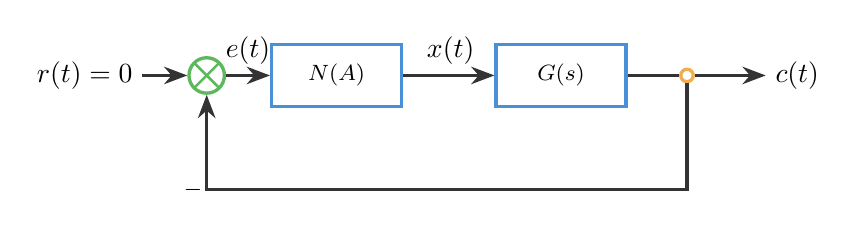
\begin{tikzpicture}[auto, >=Stealth]
  \tikzset{
    block/.style={rectangle, draw={rgb,255:red,74;green,144;blue,217}, fill=none,
      minimum width=1.65cm, minimum height=0.78cm, line width=1.2pt,
      font=\footnotesize\bfseries, align=center},
    sum/.style={circle, draw={rgb,255:red,92;green,184;blue,92}, fill=none,
      minimum size=0.45cm, line width=1.2pt,
      path picture={
        \draw[line width=0.9pt] (path picture bounding box.south west) --
          (path picture bounding box.north east);
        \draw[line width=0.9pt] (path picture bounding box.north west) --
          (path picture bounding box.south east);
      }},
    tap/.style={circle, draw={rgb,255:red,240;green,173;blue,78}, fill=none,
      minimum size=4.5pt, inner sep=0pt, line width=1.2pt},
    signal/.style={->, line width=1.2pt, draw={rgb,255:red,51;green,51;blue,51}},
    neg sign/.style={font=\footnotesize, inner sep=1pt}
  }

  \node (R) at (0,0) {$r(t)=0$};
  \node[sum] (sum) at (1.55,0) {};
  \node[block] (N) at (3.20,0) {$N(A)$};
  \node[block] (G) at (6.05,0) {$G(s)$};
  \node[tap] (tap) at (7.65,0) {};
  \node (C) at (9.05,0) {$c(t)$};

  \draw[signal] (R) -- (sum);
  \draw[signal] (sum) -- node[above] {$e(t)$} (N);
  \draw[signal] (N) -- node[above, pos=0.52] {$x(t)$} (G);
  \draw[signal] (G) -- (tap) -- (C);
  \draw[signal] (tap) |- ++(0,-1.45) -| node[neg sign, left] {$-$} (sum.south);
\end{tikzpicture}
\end{document}
